% ==============================================================================================
\section{Fault model, failover and recovery}
\label{sec:faults}

\subsection{The faults and how we inject them}

\begin{table}[!htb]
\centering\small
\caption{The faults we handle, and how each is made in the experiments.}
\label{tab:faultmodel}
\begin{tabularx}{\linewidth}{@{}P{3.3cm}LL@{}}
\toprule
Fault & How it is made & What happens \\
\midrule
A node goes silent for 1 to 20 s & The fault election (Section~\ref{sec:faultelection}), or \texttt{ctl silence}. A \emph{fault gate} in the node's network code drops all peer and client traffic and keeps memory; control messages still pass (\dlog{D13}, \dlog{D22}) & The other two drop it after 1 s and go on; it catches up and is added back \\
A node's process dies & \texttt{kill -9}, then a restart; this stands in for turning a machine off (\dlog{D265}) & The same, but it first rebuilds from its own file \\
Two nodes fail, at once or in turn & Kills and silences in every order (Section~\ref{sec:kills}) & The last node answers provisionally until it can commit (\dlog{D261}, \dlog{D262}) \\
All three fail & Kills, back together or one at a time & Each rebuilds from its own file; the longest log goes first \\
Messages lost, late, doubled & UDP and Wi-Fi do this by themselves & Retries with the same ID; first result wins \\
\bottomrule
\end{tabularx}
\end{table}

We do not handle Byzantine faults, and we did not physically pull a plug. A kill stops a process at once, as a power cut would, but it cannot lose disk writes the way a real cut can. Section~\ref{sec:limits} states this as a limit.

\subsection{Failure detection}

Every node asks every peer ``are you alive?'' each 50 ms, and any answer counts (\code{node/heartbeat.rs}, \dlog{D41}, \dlog{D79}). A peer not heard from for 20 heartbeats, so 1 s, is suspected. The shared log also watches each member's stream, every 25 ms, and counts a member silent after the same 1 s (\code{run\_detector}). Each node decides for itself, and a guess can be wrong, since a slow node looks like a dead one \cite{chandra}. A wrong guess costs a drop and a rejoin, and never two different states, because the drop below needs two nodes to agree. The heartbeats are sent to every configured peer, never only to the current members, so that two nodes that dropped each other still hear each other again.

\subsection{Failover: going on without a silent node}
\label{sec:drop}

A silent member holds up every round, because the frontier needs its stream. So the other two agree to go on without it (Figure~\ref{fig:seq-drop}). The rule that keeps this safe is that a node gives at most one promise per view, so there can be only one next view (\dlog{D252}). Every batch the silent node could have applied is at or below the cut: it applies its own batches only once a peer has saved them, and both peers stopped counting its stream before they answered.

\begin{figure}[!htb]
\centering
\begin{tikzpicture}[x=1cm,y=1cm]
  \seqactor{0}{Node 1}{-7.2}
  \seqactor{6.0}{Node 2}{-7.2}
  \seqactor[badred!10]{12.0}{Node 3\\(silent)}{-7.2}
  \seqlost{12.0}{6.0}{-0.9}{its stream stops}
  \seqself{0}{-1.4}{1 s with nothing from node 3:\\ promise itself (view 5, drop 3),\\ stop counting 3's stream}
  \seqmsg{0}{6.0}{-2.8}{Drop(view 5, node 3, I hold its stream to 210)}
  \seqself{6.0}{-3.2}{no other promise for view 5:\\ promise it, stop counting 3's stream}
  \seqrep{6.0}{0}{-4.5}{Granted(view 5, I hold it to 212, here are 211 and 212)}
  \seqself{0}{-4.9}{cut = max(210, 212) = 212}
  \seqmsg{0}{6.0}{-5.9}{DropCommit(view 5, cut 212, batches you lack)}
  \seqnote{3.0}{-6.75}{5.9}{both: remove node 3, discard its batches after 212,\\ apply what is now safe; rounds go on with nodes 1 and 2}
\end{tikzpicture}
\caption{Dropping a silent node (\code{try\_drop}, \code{on\_drop}, \code{install\_drop} in \texttt{rounds.rs}). A promise given to a peer is never taken back; without this rule, the lab PCs once made two different drops as the same view, and the digests split (\dlog{D252}).}
\label{fig:seq-drop}
\end{figure}

\subsection{Recovery: coming back}
\label{sec:rejoin}

The spec asks what state is copied, replayed or rebuilt, and how a returning node knows it is current. Figure~\ref{fig:seq-rejoin} shows the steps, and Table~\ref{tab:recovery} answers the questions.

\begin{figure}[!htb]
\centering
\begin{tikzpicture}[x=1cm,y=1cm]
  \seqactor[badred!10]{0}{Node 3\\(returning)}{-8.4}
  \seqactor{6.0}{Node 1}{-8.4}
  \seqactor{12.0}{Node 2}{-8.4}
  \seqmsg{0}{6.0}{-0.9}{Stream(my next batch)}
  \seqrep{6.0}{0}{-1.4}{NotMember(view 5)}
  \seqself{0}{-1.8}{left out: clear what it has not applied;\\ serve nothing}
  \seqmsg{0}{6.0}{-3.0}{CatchUp(from entry 840)}
  \seqrep{6.0}{0}{-3.5}{Entries(up to 4,000 commands, members, start rounds)}
  \seqself{0}{-3.9}{apply them through the state machine;\\ repeat until within 200 entries of the end}
  \seqmsg{0}{6.0}{-5.1}{Join}
  \seqself{6.0}{-5.5}{its next batch carries\\ Add(node 3, start round = round + 100)}
  \seqmsg{6.0}{12.0}{-6.5}{Stream(batch with the Add)}
  \seqnote{6.0}{-7.25}{11.6}{all members reach the Add at the same place in the order, and wait at start round $-1$;\\ node 3 has the whole log when its applied round is start round $-1$, and starts sending from there}
  \seqself{0}{-8.0}{member again: bids, plans, answers}
\end{tikzpicture}
\caption{A node comes back (\code{run\_catch\_up}, \code{on\_catch\_up}, \code{on\_join}). It is added through an entry in the shared order, so all members add it at the same place, and its new stream starts past the end of its old one (\dlog{D257}).}
\label{fig:seq-rejoin}
\end{figure}

\begin{table}[!htb]
\centering\small
\caption{The recovery protocol, against what the spec asks.}
\label{tab:recovery}
\begin{tabularx}{\linewidth}{@{}P{4.2cm}L@{}}
\toprule
The spec asks & Our answer \\
\midrule
What is copied, replayed or rebuilt? & First the node replays its own file, in the order it applied, which it saved before answering anyone (\dlog{D261}). Then a member sends what is missing, up to 4,000 commands a reply, and the node replays it through the same state machine. Its bids, suspicions and view are rebuilt from new traffic. One code path serves a silence and a restart. \\
How does it know it is current? & It asks to be added, and the members stop just before the round it starts at. It has the whole log exactly when its applied round is one before that start round, and only then does it send. A node whose log is not a start of the member's gets \code{Diverged}, writes \code{Reset} to its file, and takes the log again. \\
When does it take part again? & Its proposals are refused, and it bids, plans and answers nothing, until it is a member again (\dlog{D75}). This is checked again just before each reply, so a reply that was waiting during the fault stays quiet (\dlog{D136}). \\
\bottomrule
\end{tabularx}
\end{table}

Figure~\ref{fig:node-states} brings the pieces together as the life cycle of one node.

\begin{figure}[!htb]
\centering
\begin{tikzpicture}[x=1cm,y=1cm]
  \node[sinit] (i) at (-1.4,0) {};
  \node[state, text width=2.6cm] (start) at (1.2,0) {\textbf{Starting}\\ replays its own file};
  \node[state, text width=2.7cm, fill=mwgreen!14] (serve) at (6.4,0) {\textbf{Serving}\\ bids, plans, answers, sends its stream};
  \node[state, text width=2.7cm, fill=notefill] (deg) at (11.6,0) {\textbf{Alone}\\ answers provisionally, cannot commit};
  \node[state, text width=2.7cm, fill=badred!10] (silent) at (6.4,-3.2) {\textbf{Silent}\\ drops all traffic, keeps memory};
  \node[state, text width=2.7cm] (catch) at (1.2,-3.2) {\textbf{Catching up}\\ left out: applies the log, serves nothing};
  \node[state, text width=2.4cm, fill=black!8] (dead) at (11.6,-3.2) {\textbf{Stopped}\\ killed, memory gone};
  \draw[flow] (i) -- (start);
  \draw[flow] (start) -- node[elabel, above]{first start} (serve);
  \draw[flow] (start) -- node[elabel, left]{restart} (catch);
  \draw[flow] ([yshift=4pt]serve.east) -- node[elabel, above]{peers silent 2 s} ([yshift=4pt]deg.west);
  \draw[flow] ([yshift=-4pt]deg.west) -- node[elabel, below]{can commit again} ([yshift=-4pt]serve.west -| serve.east);
  \draw[flow] (serve) -- node[elabel, right]{fault gate closes} (silent);
  \draw[flow] (silent) -- node[elabel, above]{gate opens} (catch);
  \draw[flow] (catch.north east) -- node[elabel, sloped, above]{added back} (serve.south west);
  \draw[flow] (deg) -- node[elabel, right]{\texttt{kill -9}} (dead);
  \draw[flow] (dead.south) -- ++(0,-0.6) -| node[elabel, pos=0.25, below]{restarted with the same ID and file} (start.south west);
\end{tikzpicture}
\caption{The life of one node. Any state can go to Stopped by a kill; only one such arrow is drawn. Alone is still serving, but its answers are labelled provisional (Section~\ref{sec:degraded}).}
\label{fig:node-states}
\end{figure}

\subsection{More than one failure}
\label{sec:multi}

The class notes ask what happens with one node off and another failed, leaving one server. Our first rotating rounds could not handle two failures close together: commits stopped for the rest of the run (\dlog{D261}). Raft would have carried on in some of these cases, as long as two nodes were up, but not with one. We fixed this in four steps on the final build. Each node now saves the order it applied before answering, and rebuilds from its own file when it restarts. A member with nobody else left takes a returning node straight back, with no vote, because in a view of two nothing commits without both, so the survivor holds everything that was applied. With nobody left, the node with the longest log goes first. Figure~\ref{fig:multi} is the decision a restarted node makes.

\begin{figure}[!htb]
\centering
\begin{tikzpicture}[x=1cm,y=1cm, node distance=0.5cm]
  \node[fend] (s) {restart: replay own file, in the order applied};
  \node[fdec, below=of s] (m) {a member\\ answers?};
  \node[fdec, right=1.6cm of m] (pref) {its log a start\\ of the member's?};
  \node[fstep, right=1.1cm of pref, text width=2.6cm] (reset) {write \code{Reset}, take the log again};
  \node[fstep, below=0.9cm of pref, text width=3.4cm] (join) {catch up, \code{Join}; if the member is alone, it takes the node back with no vote (\code{add\_alone})};
  \node[fdec, below=of m] (others) {others reachable\\ within 3 s?};
  \node[fstep, below=of others, text width=3.4cm] (longest) {the longest log goes first (lowest ID on a tie); the others return to it};
  \node[fstep, left=1.0cm of longest, text width=2.8cm] (alone) {serve what it has, answer provisionally until it can commit};
  \node[fend, below=0.9cm of join] (back) {a member again};
  \draw[flow] (s) -- (m);
  \draw[flow] (m) -- node[elabel, above]{yes} (pref);
  \draw[flow] (pref) -- node[elabel, above]{no} (reset);
  \draw[flow] (reset) |- (join.east);
  \draw[flow] (pref) -- node[elabel, right]{yes} (join);
  \draw[flow] (m) -- node[elabel, right]{no} (others);
  \draw[flow] (others) -- node[elabel, right]{yes} (longest);
  \draw[flow] (others.west) -| node[elabel, pos=0.3, above]{no} (alone.north);
  \draw[flow] (longest.east) -- (longest.east -| join.west) |- (back.west);
  \draw[flow] (join) -- (back);
\end{tikzpicture}
\caption{What a node does after a restart (\code{run\_catch\_up}, \dlog{D261}). A node that cannot commit yet answers provisionally, so a client is never left with silence for long.}
\label{fig:multi}
\end{figure}

\subsection{One node left: provisional answers}
\label{sec:degraded}

A single node cannot commit, because the shared log needs a peer to save each batch. Waiting would leave the three client PCs with no answers, which is the opposite of what the class notes ask for. So a node alone answers anyway, with a plan it labels \code{Provisional}, and records it properly once a peer is back (\dlog{D120}, \dlog{D262}). This breaks our rule ``commit, then reply'', and we chose it knowingly: it trades consistency for availability in this one case, as the spec allows for speculative actions that are ``clearly labeled and reconciled''.

When a peer returns, the lone node replays its provisional plans through the shared log, and the first result recorded still wins. A provisional answer can therefore turn out to differ: another node may have planned the same report first, or the responder may have been taken. The client is not told (\dlog{D122}). In T2, with 300 responders, about 98\% of provisional answers ended differently on record (Section~\ref{sec:kills}), so a provisional answer here means ``someone will come'' rather than ``this responder will come''. Its answers are held in memory until replayed, so killing the lone node loses them.

\subsection{Consistency model}
\label{sec:consistency}

The spec asks for a consistency model for incidents, presence, resources, leases and offline changes. Phase 1 has incidents and responders; the rest belongs to Phase 2.

\begin{itemize}
  \item \textbf{Writes are totally ordered.} Every change to incidents and responders is a command in the shared log, applied by every node in the same order by a deterministic state machine. So all nodes pass through the same states, and equal digests at the same index show it.
  \item \textbf{An answer is durable before it is sent.} A node answers only after its result is applied, and it applies its own batch only after a peer saved it. The one exception is the labelled provisional answer above.
  \item \textbf{Conflicts are settled by order, not by clocks.} Two plans for the same report: the first in the order wins, and the second gets it back. Two reports wanting the same responder: the first in the order holds it, and the second chooses again at apply, the same way on every node (\dlog{D241}). No vector clocks are needed, because there is one order.
  \item \textbf{Reads are local.} A node answers a retry or a status read from its own copy, which may be a few rounds behind another node's. A returning node reads nothing until it is current.
  \item \textbf{No clock decides anything replicated.} The state machine reads no clock (\dlog{D30}). ``Too old'' is judged from the age the client states, so it never compares two machines' clocks (\dlog{D143}).
\end{itemize}
